% 页面设置
\documentclass[12pt, a4paper]{article} % 字号:12,纸张:A4
\usepackage[top=2.54cm, bottom=2.54cm, left=3.18cm,right=3.18cm]{geometry} % 页边距设置
% 字体设置
\usepackage[UTF8]{ctex}
\usepackage{fontspec} % 设置字体
%\setCJKmainfont{SimSun}[AutoFakeBold=true, BoldFont={SimHei}, ItalicFont={KaiTi}] % 正文字体
%\setCJKsansfont[AutoFakeBold=3]{KaiTi} % 无衬线字体
%\setCJKmonofont[AutoFakeBold=3]{SimHei} % 等宽字体
\setmainfont{Times New Roman} % 设置主字体为新罗马体
% 文本设置
\usepackage{enumerate} % 支持小标题编号
\linespread{1.5} % 行间距1.5倍
\usepackage{indentfirst}%首段缩进
\setlength{\parindent}{2em} % 首行缩进两字符
\usepackage[hidelinks]{hyperref} % 目录添加超链接
\usepackage{zhnumber} % 章节标题中文显示
\usepackage[cmyk]{xcolor} % 文字彩色显示
% 数学支持
\usepackage{amsmath} % 数学公式支持
\usepackage{amssymb} % 数学符号支持
\usepackage{bm} % 公式加粗
\usepackage{mathrsfs} % 花体字母
\usepackage{yhmath} % 更多的数学符号
% 图片设置
\usepackage{caption} % 插入图片标题
\usepackage{float} % 控制图片位置
\usepackage{subfigure} % 图片并排
\usepackage{booktabs} % 插入表格
% 表格设置
\usepackage{multirow} % 表格自动换行
\usepackage{bigstrut} % 表格间距
\usepackage{rotating} % 表格旋转
\usepackage{tabularx} % 表格宽度
\usepackage{colortbl} % 表格颜色
\usepackage{graphicx} % 表格自动宽度

\title{第六章 \ \ \ 支持向量机} % 文章标题
\author{Castor Ye} % 文章作者
\date{} % 文章时间

\begin{document} % 文档从这里开始。
\maketitle % 按照预定的模板把上面那些信息排好。
\newtheorem{definition}{定义}[section]
\newtheorem{theorem}{定理}[section]
\newtheorem{example}{例}[section]
\newtheorem{solution}{题解}
\newtheorem{algorithm}{算法}
\newtheorem{axiom}{公理}
\newtheorem{property}{性质}
\newtheorem{proposition}{命题}
\newtheorem{lemma}{引理}
\newtheorem{corollary}{推论}[section]
\newtheorem{remark}{注解}
\newtheorem{condition}{条件}
\newtheorem{conclusion}{结论}
\newtheorem{assumption}{假设}
\renewcommand{\figurename}{图} % 将图片序号改为图
\renewcommand{\tablename}{表} % 将表格序号改为表
%%%%%%%%%%%%%%%%%%%%%%%%%%%%%%%%%%%%%%%%%%%%%%%%%%%%%%%%%%%%%%%%%%%%%%%
% 文章内容从此开始

支持向量机是一种经典的二分类模型,基本模型定义为特征空间中最大间隔的线性分类器,其学习的优化目标便是间隔最大化,因此支持向量机本身可以转化为一个凸二次规划求解的问题。

\section{间隔与支持向量}

给定训练样本集 $D = \{(x_1, y_1), (x_2, y_2), \cdots, (x_m, y_m)\}, y_i \in \{-1, +1\}$,分类学习最基本的想法就是基于训练集 $D$ 在样本空间中找到一个划分超平面,将不同类别的样本分开。但是能将训练样本分开的超平面可能有很多,应该如何寻找最优超平面呢?

\begin{figure}[H]
    \centering
    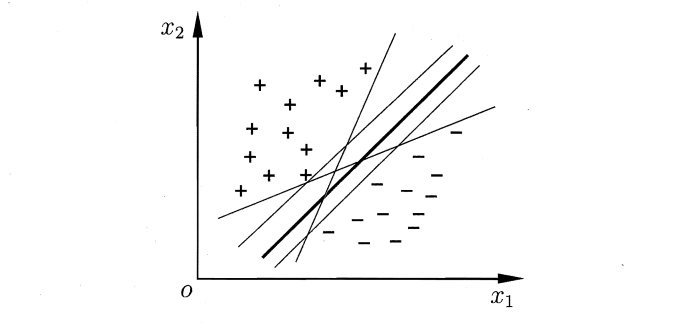
\includegraphics[width=0.8\textwidth]{../img/6-1-存在多个划分超平面将两类训练样本分开.png}
    \caption{存在多个划分超平面将两类训练样本分开}
    \label{fig:存在多个划分超平面将两类训练样本分开}
\end{figure}

直观上看,最优划分超平面所产生的结果是最鲁棒的,对未见示例的泛化能力最强。在样本空间中,我们使用线性方程来描述划分的超平面:
\begin{equation*}
    w^T x + b = 0
\end{equation*}
其中 $w = (w_1;w_2;\cdots;w_d)$ 为法向量,决定了超平面的方向;$b$ 为位移项,决定了超平面与原点之间的距离,我们将其记为 $(w, b)$。

样本空间中任意点 $x$ 到超平面 $(w, b)$ 的距离可写为:
\begin{equation*}
    r = \frac{|w^T x + b|}{||w||}
\end{equation*}

假设超平面 $(w, b)$ 能将训练样本正确分类,即对于 $(x_i, y_i) \in D$,若 $y_i = +1$,则有 $w^T x_i + b > 0$;若 $y_i = -1$,则有 $w^T x_i + b < 0$。令:
\begin{equation*}
    \left\{\begin{matrix}
        w^T x_i + b \ge 1, y_i = +1 \\
        w^T x_i + b \le 1, y_i = -1
    \end{matrix}\right.
\end{equation*}

如下图所示,距离超平面最近的这几个训练样本点使上式等号成立,它们被成为“支持向量”(support vector),两个异类支持向量到超平面距离之和为:
\begin{equation*}
    \gamma = \frac{2}{||w||}
\end{equation*}
它被称为“间隔”(margin)。

\begin{figure}[H]
    \centering
    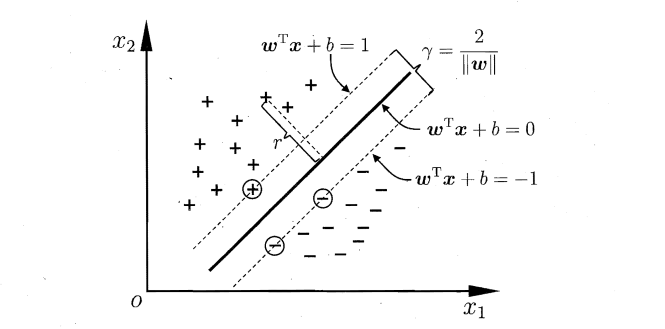
\includegraphics[width=0.8\textwidth]{../img/6-2-支持向量与间隔.png}
    \caption{支持向量与间隔}
    \label{fig:支持向量与间隔}
\end{figure}

欲找到具有“最大间隔”(maximum margin)的划分平面,也就是要找到能满足上式中约束的参数 $w$ 和 $b$,使得 $\gamma$ 最大,即:
\begin{equation*}
    \begin{array}{*{20}{l}}
        \displaystyle \min_{w, b} \frac{2}{||w||} \\
        \displaystyle s.t. \ y_i(w^T x_i + b) \ge 1, i = 1, 2, \cdots, m
    \end{array}
\end{equation*}
这就是支持向量机(Support Vector Machine, SVM)的基本型。

\section{对偶问题}

在上一节中我们得到了一个带约束的凸二次规划问题,我们求解可以得到最大间隔划分超平面所对应的模型:
\begin{equation*}
    f(x) = w^T x + b
\end{equation*}
其中 $w$ 和 $b$ 是模型参数。这个过程可以直接使用现成的优化计算包求解,但我们可以使用更高效的方法。一般我们将原问题变换为它的对偶问题,接着再对其对偶问题进行求解。为什么通过对偶问题进行求解,有下面两个原因:

\begin{enumerate}[\hspace*{2em} i.]
    \item 使用对偶问题更容易求解。
    \item 通过对偶问题求解出现了向量内积的形式,从而能更加自然地引出核函数。
\end{enumerate}

对偶问题,顾名思义,可以理解成优化等价的问题,更一般地,是将一个原始目标函数的最小化转化为它的对偶函数最大化的问题。对于当前的优化问题,首先我们写出它的朗格朗日函数:
\begin{equation*}
    L(w, b, \alpha) = \frac{1}{2} ||w||^2 + \sum_{i = 1}^{m} \alpha_i (1 - y_i(w^T x_i + b))
\end{equation*}
其中 $\alpha = (\alpha_1; \alpha_2; \cdots, \alpha_m$,令 $L(w, b, \alpha)$ 对 $w$ 和 $b$ 的偏导为零可得:
\begin{equation*}
    w = \sum_{i = 1}^{m} \alpha_i y_i x_i, \ \ \ 0 = \sum_{i = 1}^{m} \alpha_i y_i
\end{equation*}

将上式代入,即可将 $L(w, b, \alpha)$ 中的 $w$ 和 $b$ 消去,再考虑其中约束条件,就得到了对偶问题:
\begin{equation*}
    \begin{array}{*{20}{l}}
        \displaystyle \max_{\alpha} \sum_{i = 1}^{m} \alpha_i - \frac{1}{2} \sum_{i = 1}^{m} \sum_{j = 1}^{m} \alpha_i \alpha_j y_i y_j x_i ^T x_j \\
        \displaystyle s.t. \ \sum_{i = 1}^{m} \alpha_i y_i = 0, \alpha_i \ge 0, i = 1, 2, \cdots, m
    \end{array}
\end{equation*}
解出 $\alpha$ 后,求出 $w$ 和 $b$ 即可得到模型:
\begin{equation*}
    f(x) = \sum_{i = 1}^{m} \alpha_i y_i x_i^T x + b
\end{equation*}

其中:
\begin{equation*}
    \begin{array}{*{20}{l}}
        \displaystyle w = \sum_{i = 1}^{m} \alpha_i y_i x_i \\
        \displaystyle b = \frac{
            \displaystyle \max_{i: y_i = -1} w^T x_i + \min_{i: y_i = +1} w^T x_i
        }{2}
    \end{array}
\end{equation*}

从对偶问题解出的 $\alpha_i$ 是拉格朗日乘子,它对应着训练样本 $(x_i, y_i)$。注意到上式中还存在不等式约束,因此上述过程需满足 KKT(Karush-Kuhn-Tucker)条件,即:
\begin{equation*}
    \left\{\begin{matrix}
        \alpha_i \ge 0       \\
        y_i f(x_i) - 1 \ge 0 \\
        \alpha_i (y_i f(x_i) - 1) = 0
    \end{matrix}\right.
\end{equation*}
于是,对任意训练样本 $(x_i, y_i)$,总有 $\alpha_i = 0$ 或 $y_i f(x_i) = 1$。若 $\alpha_i = 0$,则该样本将会在最终模型的求和中出现,也就不会对 $f(x)$ 有任何影响;若 $\alpha_i > 0$,则必有 $y_i f(x_i) = 1$,所对应的样本点对于最大间隔边界上,是一个支持向量。这显示出支持向量机的一个重要性质:训练完成后,大部分的训练样本都不需要保留,最终模型仅与支持向量有关。

对于如何求解出 $\alpha_i$,我们引入SMO(Sequential Minimal Optimization)算法。SMO 的基本思路是先固定 $\alpha_i$ 之外的所有参数,然后求 $\alpha_i$ 上的极值。由于存在约束 $\displaystyle \sum_{i = 1}^{m} \alpha_i y_i = 0$,若固定 $\alpha_i$ 之外的其他变量,则 $\alpha_i$ 可由其他变量导出。于是,SMO 每次选择两个变量 $\alpha_i$ 和 $\alpha_j$,并固定其参数。这样,在参数初始化后,SMO 不断执行如下两个步骤直至收敛:
\begin{enumerate}[\hspace*{2em} i.]
    \item 选取一对需更新的变量 $\alpha_i$ 和 $\alpha_j$。
    \item 固定 $\alpha_i$ 和 $\alpha_j$ 以外的参数,求解模型后获得更新后的 $\alpha_i$ 和 $\alpha+j$。
\end{enumerate}

\section{核函数}

在前面的讨论中,我们假设训练样本是线性可分的,及存在一个划分平面能将训练样本正确分类。然而在现实任务中,原始样本空间内也许并不存在一个能正确划分两类样本的超平面,如下图中的“异或”问题就不是线性可分的:

\begin{figure}[H]
    \centering
    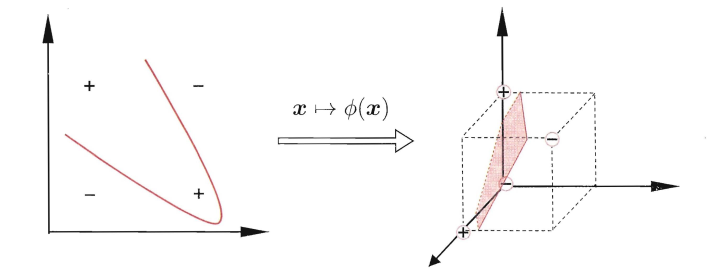
\includegraphics[width=0.8\textwidth]{../img/6-3-异或问题与非线性映射.png}
    \caption{异或问题与非线性映射}
    \label{fig:异或问题与非线性映射}
\end{figure}

对这样的问题,可将样本从原始空间映射到一个更高维的特征空间,使得样本在这个特征空间内线性可分。

令 $\phi (x)$ 表示将 $x$ 映射后的特征向量,于是,在特征空间中划分超平面所对应的模型可表示为:
\begin{equation*}
    f(x) = w^T \phi(x) + b
\end{equation*}
其中 $w$ 和 $b$ 是模型参数,有:
\begin{equation*}
    \begin{array}{*{20}{l}}
        \displaystyle \min_{w, b} \frac{2}{||w||} \\
        \displaystyle s.t. \ y_i(w^T \phi(x_i) + b) \ge 1, i = 1, 2, \cdots, m
    \end{array}
\end{equation*}

则其对偶问题是:
\begin{equation*}
    \begin{array}{*{20}{l}}
        \displaystyle \max_{\alpha} \sum_{i = 1}^{m} \alpha_i - \frac{1}{2} \sum_{i = 1}^{m} \sum_{j = 1}^{m} \alpha_i \alpha_j y_i y_j \phi(x_i) ^T \phi(x_j) \\
        \displaystyle s.t. \ \sum_{i = 1}^{m} \alpha_i y_i = 0, \alpha_i \ge 0, i = 1, 2, \cdots, m
    \end{array}
\end{equation*}

为求解 $\phi(x_i) ^T \phi(x_j)$,我们设想这样一个函数:
\begin{equation*}
    \kappa (x_i, x_j) = <\phi(x_i), \phi(x_j)> = \phi(x_i) ^T \phi(x_j)
\end{equation*}

用该函数重写对偶问题后并求解,得到:
\begin{equation*}
    f(x) = \sum_{i = 1}^{m} \alpha_i y_i \kappa(x, x_i) + b
\end{equation*}

这里的函数 $\kappa (\cdot, \cdot)$ 就是“核函数”(kernel function)。上式显示出模型最优解可通过训练样本的核函数展开,这一展示亦称“支持向量展示”(support vector expansion)。那么,如何确定核函数呢?核函数是否一定存在呢?

\begin{theorem}\label{theorem:核函数}
    核函数:令 $X$ 为输入空间,$\kappa (\cdot, \cdot)$ 是定义在 $X \times X$ 上的对称函数,则 $\kappa$ 是核函数当且仅当对于任意数据 $D = \{x_1, x_2,\cdots, x_m\}$,“核矩阵”(kernel matrix)$K$ 总是半正定的:
    \begin{equation*}
        K = \left[ {\begin{array}{*{20}{c}}
                        \kappa (x_1, x_1) & \cdots & \kappa(x_1, x_j)  & \cdots & \kappa(x_1, x_m) \\
                        \vdots            & \ddots & \vdots            & \ddots & \vdots           \\
                        \kappa (x_i, x_1) & \cdots & \kappa(x_i, x_j)  & \cdots & \kappa(x_i, x_m) \\
                        \vdots            & \ddots & \vdots            & \ddots & \vdots           \\
                        \kappa (x_m, x_1) & \cdots & \kappa (x_m, x_j) & \cdots & \kappa(x_m, x_m) \\
                    \end{array}} \right]
    \end{equation*}
\end{theorem}

定理 \ref{theorem:核函数} 中表明,只要一个对称函数所对应的和矩阵半正定,它就能作为核函数使用。事实上,任何一个核函数都隐式地定义了一个称为“再生核希尔伯特空间”(Reproducing Kernel Hilbert Space, RKHS)的特征空间。

\begin{figure}[H]
    \centering
    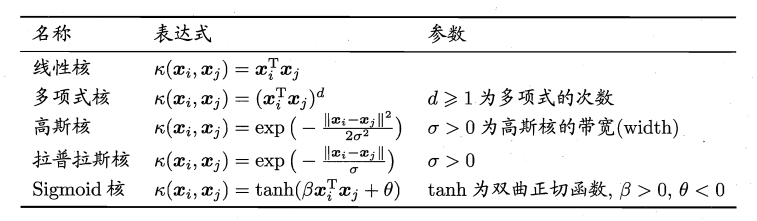
\includegraphics[width=0.8\textwidth]{../img/6-4-常用核函数.png}
    \caption{常用核函数}
    \label{fig:常用核函数}
\end{figure}

此外,还可通过函数组合得到,例如:
\begin{enumerate}[\hspace*{2em} i.]
    \item 若 $\kappa_1$ 和 $\kappa_2$ 为核函数,则对于任意正数 $\gamma_1, \gamma_2$,其线性组合 $\gamma_1 \kappa_1 + \gamma_2 \kappa_2$ 也是核函数。
    \item 若 $\kappa_1$ 和 $\kappa_2$ 为核函数,则核函数的直积 $\kappa_1 \otimes \kappa_2 (x, z) = \kappa_1 (x, z) \kappa_2 (x, z)$ 也是核函数。
    \item 若 $\kappa_1$ 为核函数,则对于任意函数 $g(x)$,$\kappa (x, z) = g(x) \kappa_1 (x, z) g(z)$ 也是核函数。
\end{enumerate}

\section{软间隔与正则化}

即使我们已经有了核函数,但实际上我们依然很难确定合适的核函数使得训练样本在特征空间中线性可分,即使存在线性可分,也可能是过拟合造成的。

缓解该问题的一个办法是允许支持向量机在一些样本上出错,即引入“软间隔”(soft margin)的概念。

\begin{figure}[H]
    \centering
    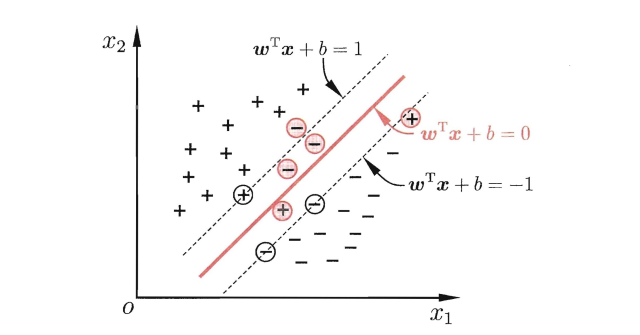
\includegraphics[width=0.8\textwidth]{../img/6-5-软间隔示意图.png}
    \caption{软间隔示意图,红色圈出了一些不满足约束的样本}
    \label{fig:软间隔示意图}
\end{figure}

软间隔允许某些样本不满足约束:
\begin{equation*}
    y_i(w^T x_i + b) \ge 1
\end{equation*}
在最大化间隔的同时,不满足约束的样本应尽可能少。于是,优化目标可以写为:
\begin{equation*}
    \min_{w, b} \frac{1}{2} ||w||^2 + C \sum_{i = 1}^{m} \ell_{0 / 1} (y_i (w^T x_i + b) - 1)
\end{equation*}
其中 $C > 0$ 是一个常数,$\ell_{0 / 1}$ 是“$0 / 1$ 损失函数”:
\begin{equation*}
    \ell_{0 / 1}(z) = \left\{\begin{matrix}
        1, if z < 0 \\
        0, otherwise
    \end{matrix}\right.
\end{equation*}
显然,当 $C$ 为无穷大时,所有样本均满足约束;当 $C$ 取有限值时,允许一些样本不满足约束。

然而,$\ell_{0 / 1}$ 非凸、非连续,数学性质不好,因此我们一般用其他“替代损失”(surrogate loss):

\begin{enumerate}[\hspace*{2em} i.]
    \item hinge 损失:$\ell_{hinge} (z) = \max (0, 1 - z)$
    \item 指数损失(exponential loss):$\ell_{exp} (z) = \exp (-z)$
    \item 对率损失(logistic loss):$\ell_{log} (z) = \log(1 + \exp(-z))$
\end{enumerate}

\begin{figure}[H]
    \centering
    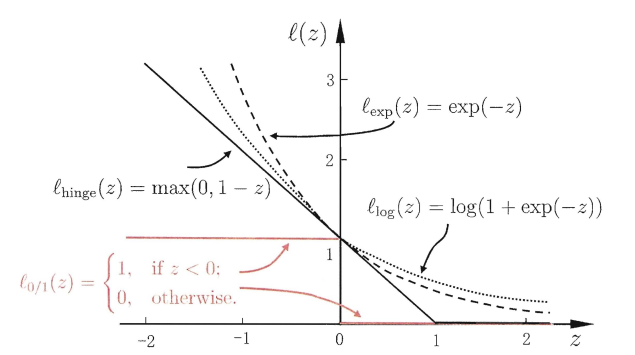
\includegraphics[width=0.8\textwidth]{../img/6-6-三种常见的替代损失函数.png}
    \caption{三种常见的替代损失函数}
    \label{fig:三种常见的替代损失函数}
\end{figure}

若采用 hinge 损失,则有:
\begin{equation*}
    \min_{w, b} \frac{1}{2} ||w||^2 + C \sum_{i = 1}^{m} \max(0, 1 - y_i (w^T x_i + b))
\end{equation*}

引入“松弛变量”(slack variables) $\xi_i \ge 0$,可将上式重写为:
\begin{equation*}
    \begin{array}{*{20}{l}}
        \displaystyle \min_{w, b, \xi_i} \frac{1}{2} ||w||^2 + C \sum_{i = 1}^{m} \xi_i \\
        \displaystyle s.t. \ y_i (w^T x_i + b) \ge 1 - \xi_i, \xi_i \ge 0, i = 1, 2, \cdots, m
    \end{array}
\end{equation*}
这就是常用的“软间隔支持向量机”。

\section{支持向量回归}

给定训练样本 $D = \{(x_1, y_1), (x_2, y_2), \cdots, (x_m, y_m)\}, y_i \in \mathbb{R}$,希望学得一个回归模型,使得 $f(x)$ 与 $y$ 尽可能接近,$w$ 和 $b$ 都是待确定的模型参数。

支持向量回归(Support Vector Regression, SVR)假设我们能容忍 $f(x)$ 与 $y$ 之间最多有 $\epsilon$ 的偏差,即仅当 $f(x)$ 与 $y$ 之间的差别绝对值大于 $\epsilon$ 时才计算损失。如下图所示,这相当于以 $f(x)$ 为中心,构建了一个宽度为 $2 \epsilon$ 的间隔带,若训练样本落入此间隔带,则认为是被预测正确的。

\begin{figure}[H]
    \centering
    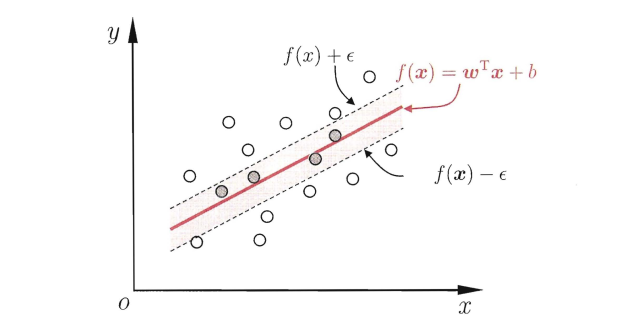
\includegraphics[width=0.8\textwidth]{../img/6-7-支持向量回归示意图.png}
    \caption{支持向量回归示意图}
    \label{fig:支持向量回归示意图}
\end{figure}

\section{核方法}

从上面可以发现,给定训练样本 $D = \{(x_1, y_1), (x_2, y_2), \cdots, (x_m, y_m)\}$,若不考虑偏移项 $b$,则无论 SVM 还是 SVR,学得的模型总能表示成核函数 $\kappa (x, x_i)$ 的线性组合。

\begin{theorem}
    表示定理:另 $\mathbb{H}$ 为核函数 $\kappa$ 对应的再生希尔伯特空间,$||h||_{\mathbb{H}}$ 表示 $\mathbb{H}$ 空间中关于 $h$ 的范数,对于任意单调递增函数 $\Omega: [0, \infty] \to \mathbb{R}$ 和任意非负损失函数 $\ell : \mathbb{R}^m \to [0, \infty]$,优化问题:
    \begin{equation*}
        \min_{h \in \mathbb{H}} F(h) = \Omega (||h||_{\mathbb{H}}) + \ell (h(x_1), h(x_2), \cdots, h(x_m))
    \end{equation*}
    的解总可写为:
    \begin{equation*}
        h^* (x) = \sum_{i = 1}^{m} \alpha_i \kappa(x, x_i)
    \end{equation*}
\end{theorem}

人们发展出一系列基于核函数的学习方法,统称为“核方法”(kernel methods)。

\end{document}